% !TeX program = pdfLaTeX
\documentclass[12pt]{article}
\usepackage{amsmath}
\usepackage{graphicx,psfrag,epsf}
\usepackage{enumerate}
\usepackage{natbib}
\usepackage{textcomp}
\usepackage[hyphens]{url} % not crucial - just used below for the URL
\usepackage{hyperref}
\providecommand{\tightlist}{%
  \setlength{\itemsep}{0pt}\setlength{\parskip}{0pt}}

%\pdfminorversion=4
% NOTE: To produce blinded version, replace "0" with "1" below.
\newcommand{\blind}{0}

% DON'T change margins - should be 1 inch all around.
\addtolength{\oddsidemargin}{-.5in}%
\addtolength{\evensidemargin}{-.5in}%
\addtolength{\textwidth}{1in}%
\addtolength{\textheight}{1.3in}%
\addtolength{\topmargin}{-.8in}%

%% load any required packages here


\usepackage{color}
\usepackage{fancyvrb}
\newcommand{\VerbBar}{|}
\newcommand{\VERB}{\Verb[commandchars=\\\{\}]}
\DefineVerbatimEnvironment{Highlighting}{Verbatim}{commandchars=\\\{\}}
% Add ',fontsize=\small' for more characters per line
\usepackage{framed}
\definecolor{shadecolor}{RGB}{248,248,248}
\newenvironment{Shaded}{\begin{snugshade}}{\end{snugshade}}
\newcommand{\AlertTok}[1]{\textcolor[rgb]{0.94,0.16,0.16}{#1}}
\newcommand{\AnnotationTok}[1]{\textcolor[rgb]{0.56,0.35,0.01}{\textbf{\textit{#1}}}}
\newcommand{\AttributeTok}[1]{\textcolor[rgb]{0.77,0.63,0.00}{#1}}
\newcommand{\BaseNTok}[1]{\textcolor[rgb]{0.00,0.00,0.81}{#1}}
\newcommand{\BuiltInTok}[1]{#1}
\newcommand{\CharTok}[1]{\textcolor[rgb]{0.31,0.60,0.02}{#1}}
\newcommand{\CommentTok}[1]{\textcolor[rgb]{0.56,0.35,0.01}{\textit{#1}}}
\newcommand{\CommentVarTok}[1]{\textcolor[rgb]{0.56,0.35,0.01}{\textbf{\textit{#1}}}}
\newcommand{\ConstantTok}[1]{\textcolor[rgb]{0.00,0.00,0.00}{#1}}
\newcommand{\ControlFlowTok}[1]{\textcolor[rgb]{0.13,0.29,0.53}{\textbf{#1}}}
\newcommand{\DataTypeTok}[1]{\textcolor[rgb]{0.13,0.29,0.53}{#1}}
\newcommand{\DecValTok}[1]{\textcolor[rgb]{0.00,0.00,0.81}{#1}}
\newcommand{\DocumentationTok}[1]{\textcolor[rgb]{0.56,0.35,0.01}{\textbf{\textit{#1}}}}
\newcommand{\ErrorTok}[1]{\textcolor[rgb]{0.64,0.00,0.00}{\textbf{#1}}}
\newcommand{\ExtensionTok}[1]{#1}
\newcommand{\FloatTok}[1]{\textcolor[rgb]{0.00,0.00,0.81}{#1}}
\newcommand{\FunctionTok}[1]{\textcolor[rgb]{0.00,0.00,0.00}{#1}}
\newcommand{\ImportTok}[1]{#1}
\newcommand{\InformationTok}[1]{\textcolor[rgb]{0.56,0.35,0.01}{\textbf{\textit{#1}}}}
\newcommand{\KeywordTok}[1]{\textcolor[rgb]{0.13,0.29,0.53}{\textbf{#1}}}
\newcommand{\NormalTok}[1]{#1}
\newcommand{\OperatorTok}[1]{\textcolor[rgb]{0.81,0.36,0.00}{\textbf{#1}}}
\newcommand{\OtherTok}[1]{\textcolor[rgb]{0.56,0.35,0.01}{#1}}
\newcommand{\PreprocessorTok}[1]{\textcolor[rgb]{0.56,0.35,0.01}{\textit{#1}}}
\newcommand{\RegionMarkerTok}[1]{#1}
\newcommand{\SpecialCharTok}[1]{\textcolor[rgb]{0.00,0.00,0.00}{#1}}
\newcommand{\SpecialStringTok}[1]{\textcolor[rgb]{0.31,0.60,0.02}{#1}}
\newcommand{\StringTok}[1]{\textcolor[rgb]{0.31,0.60,0.02}{#1}}
\newcommand{\VariableTok}[1]{\textcolor[rgb]{0.00,0.00,0.00}{#1}}
\newcommand{\VerbatimStringTok}[1]{\textcolor[rgb]{0.31,0.60,0.02}{#1}}
\newcommand{\WarningTok}[1]{\textcolor[rgb]{0.56,0.35,0.01}{\textbf{\textit{#1}}}}


\usepackage{booktabs}
\usepackage{longtable}
\usepackage{array}
\usepackage{multirow}
\usepackage{wrapfig}
\usepackage{float}
\usepackage{colortbl}
\usepackage{pdflscape}
\usepackage{tabu}
\usepackage{threeparttable}
\usepackage{threeparttablex}
\usepackage[normalem]{ulem}
\usepackage{makecell}

\begin{document}


\def\spacingset#1{\renewcommand{\baselinestretch}%
{#1}\small\normalsize} \spacingset{1}


%%%%%%%%%%%%%%%%%%%%%%%%%%%%%%%%%%%%%%%%%%%%%%%%%%%%%%%%%%%%%%%%%%%%%%%%%%%%%%

\if0\blind
{
  \title{\bf Hyperparameter Tuning Strategies and Applications to Random
Forests}

  \author{
        Tony Ni \thanks{Thank you to Nick Horton for his help and
guidance in the creation of this project.} \\
    Department of Mathematics and Statistics, Amherst College\\
      }
  \maketitle
} \fi

\if1\blind
{
  \bigskip
  \bigskip
  \bigskip
  \begin{center}
    {\LARGE\bf Hyperparameter Tuning Strategies and Applications to
Random Forests}
  \end{center}
  \medskip
} \fi

\bigskip
\begin{abstract}
The performance of machine learning models heavily depend upon the
correct specification of certain variables, known as hyperparameters,
during their creation. How to best pick these hyperparameters in order
to create the most optimum model is quite difficult due to the trial and
error approach of creating ML models being quite time-consuming. As a
meta-learning problem, several popular approaches have emerged to aid in
the creation of optimal machine learning models those of which are
further discussed in this report include: grid search, random search,
and sequential model-based optimization methods. We also perform some
application studies to random forest classification problems with
certain datasets in order to compare and contrast their effectiveness
and runtimes, alongside performing a case-study on language learning
abilities.
\end{abstract}

\noindent%
{\it Keywords:} machine learning, classification, meta learning, model
parameter, hyperparameter
\vfill

\newpage
\spacingset{1.45} % DON'T change the spacing!

\hypertarget{introduction}{%
\section{Introduction}\label{introduction}}

\label{sec:intro}

Machine Learning is a rapidly evolving subfield of artificial
intelligence widely utilized by practitioners in fields ranging from
health care, sciences, government. Its ubiquity is widely due to its
practicality, especially in an era where data is more accessible and
prevalent than ever. As its name suggests, many of the techniques in
machine learning have to do with the training of a computer (machine) to
learn from data and use it to execute a program to solve a problem at
hand.

These problems can range from simple tasks such as trying to generate a
``rule'' to differentiate between groups such as apples and oranges
(classification task), trying to find unknown clusters in a set of data
(clustering), etc. It would be difficult to go into the details and
specifics within the types of learning that machine learning
encompasses, as there are far too many machine learning tasks to cover
in a single report -- but the most important takeaway would have to be
the ability of machine learning algorithms to develop, learn, and train
from data to create models.

While in the process of creating these models, it can often be
challenging to find the model which best captures the information from
the training data. Depending on what sort of machine learning task is in
question (classification, clustering, reinforcement learning, etc.) each
model takes in unique parameters known as `hyperparameters,' which
govern the training process itself.

For example, if we were looking at clustering as a technique
(specifically K-Means clustering) -- some hyperparameters to alter would
be things such as: the number of clusters we want, the initial
configuration of centroids, the max number of iterations we want the
algorithm to run, etc. \citep{Picco2016}. Altering these hyperparameters
(also known as model-specific properties) can often change how the model
fits and adheres to the training data. Thus, it is important to choose
hyperparameters that allows for the model to best adapt to the training
data without underfitting or overfitting to the data.

How do we pick the correct configuration of parameters to use then? The
process of creating these models itself is a sub-field known as
``meta-learning,'' and many techniques have been founded and developed
to tackle the challenges of finding the best model for a given task. One
of the most notable methods of meta-learning tasks is known as
``hyperparameter tuning,'' which will be the focus of this report. For
those interested in a more in-depth exploration of other topics in meta
learning, please refer to: \citep{Hutter2014}, \citep{Vanschoren2018},
and \citep{Reif2012}.

Hyperparameter tuning is essentialy an optimization task, in which we
are trying to look for the best combinations of hyperparameters to use
to train our model. Methods such as grid search, random search, and
Bayesian searches have come up in recent times which aid machine
scientists to obtain the set of hyperparameters which builds the best
performing model.

\hypertarget{question}{%
\section{Question}\label{question}}

\label{sec:question}

The focus of my project specifically encompasses hyperparameter tuning
and optimization with regards to ensemble-learning algorithms --
specifically classification with random forests, and studying the
effectiveness of three different hyperparameter tuning techniques: grid
search, random search, and Bayesian hyperparameter optimization -- with
regards to large data.

\hypertarget{background}{%
\section{Background}\label{background}}

\label{sec:background}

\hypertarget{model-parameters-and-hyperparameters}{%
\subsection{Model Parameters and
Hyperparameters}\label{model-parameters-and-hyperparameters}}

\label{sec:param_hyperparam}

An important conceptualization of a model parameter and hyperparameter
is essential to understanding the underpinnings of model tuning and
meta-learning. These are terms which are often confused for one another
in machine learning. A \emph{model parameter}, in terms of machine
learning algorithms, is a variable whose value is estimated from the
dataset, \emph{not} by the user. For example, the coefficients/effects
of the explanatory variables in a linear regression model are known as
model parameters. Some other model parameters in machine learning
include weights and biases which are important to the functioning of
neural networks \citep{Yang2020}.

A hyperparameter on the other hand is a variable whose value is set by
the user before the model training begins. These values can freely be
adjusted by the user in order to obtain different models, and as such,
it is important to set model parameters correctly in order to obtain
models with optimal performance. An example of a model hyperparameter
includes variables such as \(k\) (the number of clusters) in a
clustering algorithm.

Misspecification of model hyperparameters are detrimental to machine
learning models' performance. If we think about clustering as a
technique we wish to run in order to differentiate between different
types of fruits (say, apples and oranges), it is important to specify a
logical number of clusters to find. Assuming that the dataset only has
information on the most common fruits in the U.S., values between 10 or
20 seem to be reasonable. We don't really expect to find more than 20
different fruits in our dataset. Some unreasonable values one might set
the number of clusters to find, \(k\), such as 1000 would be
unreasonable due to it not making sense in the context of the situation.
If this were the case, the model clearly would not be able to find the
correct clusters in the data due to misspecification of the number of
clusters \(k\).

However, how would the user know what values are the most optimal to
pick in order to achieve the most optimum level? This is where
hyperparameter tuning can assist us.

\hypertarget{hyperparameter-tuning}{%
\subsection{Hyperparameter Tuning}\label{hyperparameter-tuning}}

\label{sec:tuning}

Hyperparameter tuning works in a variety of ways but it generally
involves running an algorithm in order to find the combination of
optimum combinations of hyperparameters and the methods to do have are
varied and differ in their approaches. The core of all tuning algorithms
involves running multiple trials with a variety of combinations of
hyperparameters and identifying which combination minimizes (or
maximizes) the loss function metric the user specifies (accuracy,
misclassification rate, etc.).

To get a better sense of things (i.e, why hyperparameter tuning is
important/helpful), the following section will discuss how
hyperparameter tuning with regards to classification trees. In
classification, our goal is of course, to create a model which is able
to predict which class a certain observation belongs to. An example
classification task will be performed with the \texttt{palmerpenguins}
dataset which contains observations regarding body measurements and
other supplementary information for 344 penguins collected from the
Palmer Archipelago. The classification task at hand will be to create a
classification tree model which is able to predict the \texttt{species}
from the following ``Adelie,'' ``Gentoo,'' and ``Chinstrap'' penguins
which comprise the dataset.

The difficulty in creating classification tree models which are
meaningful lies in the splitting and pruning the trees itself. First and
foremost, trees generally perform splits on variables in order to
differentiate between classes. For example in our
\texttt{palmerpenguins} dataset, we may want to create a split on the
variable \texttt{bill\_length\_mm} and claim that a
\texttt{bill\_length\_mm} of \textless{} 40 usually means that the
penguin is an ``Adelie'' penguin, and those with
\texttt{bill\_length\_mm} \textgreater= 40 usually are ``Gentoo'' and
``Chinstrap'' penguins. In general, splits in which the groups are
mostly pure are the most ideal -- if a node is 100\% pure, it means that
all observations in that node belong to the same class.

In creating a classification tree model, it is possible to specify
\texttt{minsplit}, the minimum number of observations which must exist
in a node in order for a split to be attempted, \texttt{minbucket}, the
minimum number of observations in any terminal/leaf node, etc. These are
the hyperparameters for creating a decision tree.

We will create and feature two unique decision tree models for the
\texttt{palmerpenguins} data set using distinct combinations for
\texttt{minsplit} and \texttt{minbucket} to show how the model output
can vary with a slight tweak to these values.

\newpage

\begin{figure}
\centering
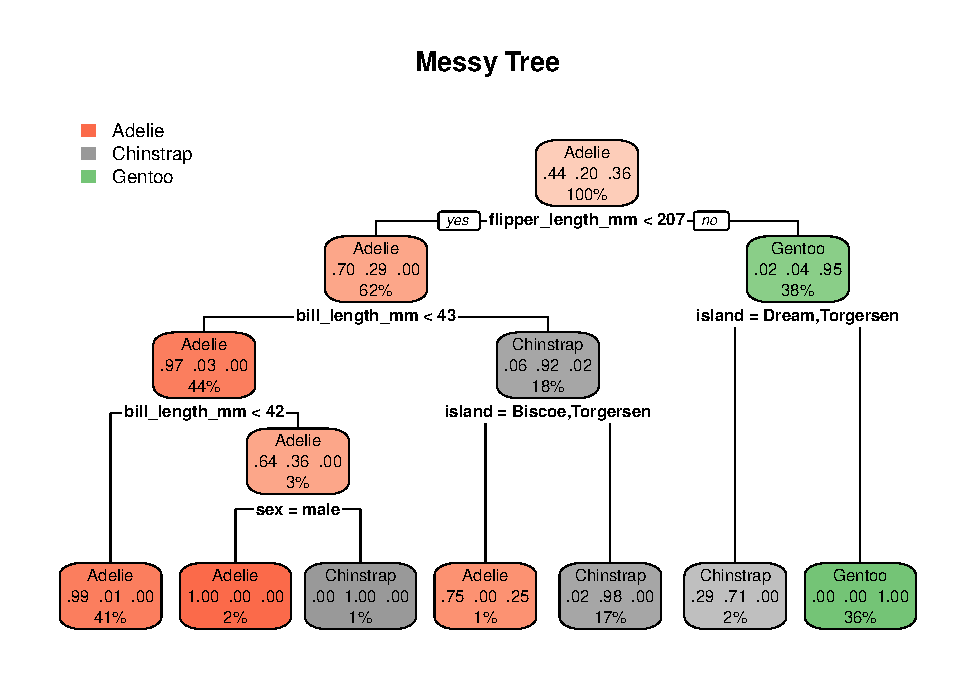
\includegraphics{report_files/figure-latex/tree1.1-1.pdf}
\caption{\label{fig:tree1.1} An classification tree created using the
hyperparameters of \texttt{minsplit} = 2 and \texttt{minbucket} = 2}
\end{figure}

The first classification tree shown in figure \ref{fig:tree1.1} was
created used a \texttt{minsplit} = 10 and \texttt{minbucket} = 2. The
following rules set by these hyperparameter dictates the following:
while creating the tree, the algorithm only splits a node if it has more
than 10 observations in it, and if a split would create a new node with
less than 2 observations. Due to the \texttt{minsplit} value being
rather small, the algorithm will be quite liberal with splitting nodes
(it keeps splitting nodes if they have more than 10 observations), and
also is quite generous with what sort of nodes are being created (nodes
of size 2 or larger are deemed fine to make). This is obviously quite
troublesome as the values that we set for these hyperparameters yield
which is rather descriptive and difficult to interpret as it seems to
overfit the data tremendously.

To give a expository explanation as to how to interpret this
classification tree for those who may be unfamiliar with it: starting
from the the root (top-most) node, once traverses down the down while
asking the question at each split, and then going left or right
depending on the answer. For example, ``Is \texttt{flipper\_length\_mm}
\(<\) 207?'' If yes, we travel down the left of the split and proceed to
the next question. The numbers inside each node specify the proportion
of each type of penguin which fell into this node depending on the
specifications of the model. For example, we can see that 70\% of Adelie
penguins, 29\% of Chinstrap penguins, and 0\% of Gentoo penguins have a
\texttt{flipper\_length\_mm} \(<\) 207.

Altering the hyperparameters to have \texttt{minsplit} = 30, and
\texttt{minbucket} = 15, to obtain a new tree then, will yield:

\begin{figure}
\centering
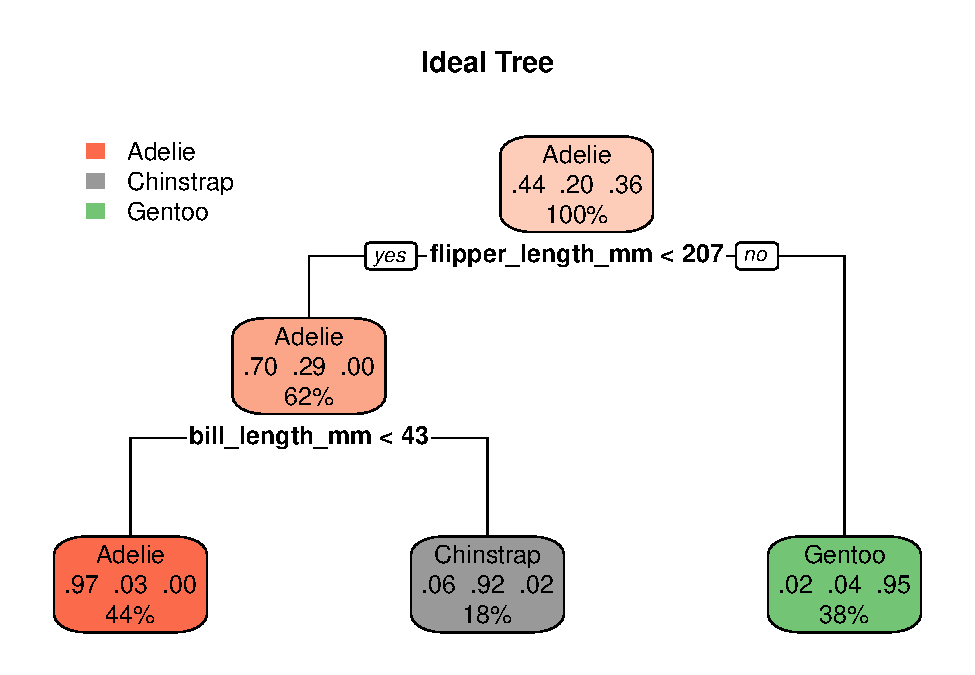
\includegraphics{report_files/figure-latex/tree2.1-1.pdf}
\caption{\label{fig:tree2.1} An classification tree created using the
hyperparameters of \texttt{minsplit} = 30 and \texttt{minbucket} = 15}
\end{figure}

In the tree shown in \ref{fig:tree2.1}tree, more reasonable values of
\texttt{minsplit} and \texttt{minbucket} are chosen, in which a split is
considered if a node has observations \(\ge\) 30, and if a split would
make a node that has less than 15 observations, it won't split the node.
The second set of hyperparameters yields a tree which isn't as
overfitted as seen in the first tree, as a result of picking good
hyperparameter values.

Thus from this in-depth study on classification trees and the
hyperparameters which dictate the algorithm's behavior in creating a
decision tree model, it can be seen that picking good hyperparamter
values is essential -- not just for decision tree model making, but all
types of machine learning models also. It can be quit troublesome to
determine what sorts of hyperparameter values to pick, and that fact
compounded by the myriad of machine learning techniques out there makes
it quite bothersome to have to go through multiple combinations of
hyperparameter values in a model just to see which one is the most
optimum, which is why hyperparameter optimization/tuning is essential.

A more in-depth discussion on how the hyperparameter methods perform and
work will be discussed in the methods section \ref{sec:methods}.

\newpage

\hypertarget{methods}{%
\section{Methods}\label{methods}}

\label{sec:methods}

Grid search (which will be implemented with the \texttt{caret} package
in R) is a brute-force/exhaustive algorithm where the user specifies a
list of values for hyperparameters and the computer evaluates the
performance of each combination, which allows us to observe the most
optimum combination of values. Although this method guarantees that the
most optimal configuration of hyperparameters will be found at the
search's conclusion, the issue lies in the runtime. As a brute force
approach whose runtime is dependent on the number of hyperparameters
given, we can expect the time-complexity of this approach to be quite
abysmal. Grid search has been found to be reliable in low dimensional
spaces however, and is simple to implement in cases when the
dimensionality of a dataset is low \citep{Bergstra2012}.

The idea of random search is quite similar to grid search, but instead
of evaluating each combination of hyperparameters like grid search does,
random search evaluates random combinations of a range hyperparameter
values until a criteria is met (like the maximum number of iterations
being reached). Random search will also be implemented using the
\texttt{caret} package in R. While random search sacrifices the
comprehensibility (looking every possible combination of
hyperparameters) of grid search, its runtime is far more feasible. Where
it falls short however is that due to the combinations being selected by
random chance, it can often yield high variance during computing.
Everything is being left to luck, which is quite risky
\citep{Bergstra2012}.

The most recent advances in hyperparameter tuning is Bayesian
hyperparameter optimization which as its name suggests, utilizes
Bayesian logic in order to select the most promising hyperparameters.
The specific type of Bayesian hyperparameter optimziation technique we
will be observing is the Sequential Model-based Optimization (with the
\texttt{tuneranger} package in R) which creates and evaluates models
based on previous iterations and chooses future combinations while
considering for these results. Essentially, with the line of Bayesian
reasoning, with more runs and combinations -- the model will eventually
become ``less wrong,'' and will settle on the best combination of
hyperparameters in fewer iterations that both grid search and random
search \citep{Probst2019}.

Sequential Model-Based Optimization essentially consists of the
following steps:

\begin{enumerate}
\def\labelenumi{\arabic{enumi})}
\item
  Specify an evaluation metric to use (RMSE, accuracy), evaluation
  strategy to test the model on (bagging, CV), and hyperparameters you
  wish to use in creating the model in question and create your initial
  model.
\item
  Based on the output from step 1, fit a regression model (also known as
  a surrogate model) on all previously tested hyperparameters with the
  y-axis as the evaluation measure and hyperparameters as the x-axis
\item
  Based on the regression model in step 2, choose a new combination of
  hyperparameters with good performance metrics to create an updated
  model, evaluate the updated model, and then add it to the existing
  hyperparameter space.
\item
  Repeat steps 2-3 until a desired model is reached \citep{Probst2019}.
\end{enumerate}

The focus on the differences between these methods thus lie in their
runtimes. Each method will be able to find a combination of
hyperparameters which yield the most optimum model in accordance with
their principles, but the problem lies in how quickly these combinations
can be obtained alongside their ease of implementation and effectiveness
\citep{Probst2019}

\newpage

\hypertarget{example-cells}{%
\section{Example: Cells}\label{example-cells}}

\label{sec:cells}

To begin our investigation on the implementations of the tuning
algorithms, we will introduce \texttt{cells} a dataset which is featured
in the package \texttt{modeldata}, which contains information on cell
segmentation imaging -- with observations belonging to two classes
\texttt{WS}, well-segmented and \texttt{PS} poorly-segmented.

Each of the three aforementioned techniques will be implemented with
regards to creating a random forest classification model of the
\texttt{cells} dataset. A careful consideration of the runtimes and
effectiveness of each of the three methods will further be discussed as
well. In each implementation of the methods discussed, the length it
will take for the tuning algorithm to finish will be measured, to give a
sense of the feasbility of implementation of each respective method
towards a large-scale application to big data.

First, we will be implementing grid search as a means to find optimal
hyperparameters for our random forest.

\begin{verbatim}
## Random Forest 
## 
## 1414 samples
##   56 predictor
##    2 classes: 'PS', 'WS' 
## 
## No pre-processing
## Resampling: Cross-Validated (10 fold, repeated 3 times) 
## Summary of sample sizes: 1273, 1272, 1272, 1273, 1273, 1272, ... 
## Resampling results across tuning parameters:
## 
##   mtry  min.node.size  splitrule   Accuracy   Kappa    
##   2     1              gini        0.8208138  0.6057310
##   2     1              extratrees  0.8184497  0.5989964
##   2     2              gini        0.8243499  0.6139725
##   2     2              extratrees  0.8160840  0.5930653
##   2     3              gini        0.8234009  0.6121283
##   2     3              extratrees  0.8172727  0.5944846
##   2     4              gini        0.8219908  0.6082599
##   2     4              extratrees  0.8210568  0.6034409
##   2     5              gini        0.8212799  0.6067697
##   2     5              extratrees  0.8151483  0.5898296
##   3     1              gini        0.8245713  0.6149485
##   3     1              extratrees  0.8234026  0.6105288
##   3     2              gini        0.8243449  0.6147515
##   3     2              extratrees  0.8207988  0.6055935
##   3     3              gini        0.8248127  0.6159866
##   3     3              extratrees  0.8231662  0.6093750
##   3     4              gini        0.8236373  0.6121643
##   3     4              extratrees  0.8252905  0.6149139
##   3     5              gini        0.8236423  0.6131679
##   3     5              extratrees  0.8184480  0.5993792
##   4     1              gini        0.8257550  0.6186003
##   4     1              extratrees  0.8219842  0.6078107
##   4     2              gini        0.8241052  0.6147956
##   4     2              extratrees  0.8233909  0.6120347
##   4     3              gini        0.8267040  0.6206822
##   4     3              extratrees  0.8219825  0.6075990
##   4     4              gini        0.8238737  0.6138257
##   4     4              extratrees  0.8257750  0.6166705
##   4     5              gini        0.8241035  0.6147879
##   4     5              extratrees  0.8236457  0.6111562
##   5     1              gini        0.8262311  0.6201798
##   5     1              extratrees  0.8259964  0.6181764
##   5     2              gini        0.8262311  0.6194586
##   5     2              extratrees  0.8255269  0.6171010
##   5     3              gini        0.8292878  0.6264271
##   5     3              extratrees  0.8271651  0.6205325
##   5     4              gini        0.8245763  0.6167361
##   5     4              extratrees  0.8259897  0.6181006
##   5     5              gini        0.8245763  0.6167174
##   5     5              extratrees  0.8243449  0.6138758
## 
## Accuracy was used to select the optimal model using the largest value.
## The final values used for the model were mtry = 5, splitrule = gini
##  and min.node.size = 3.
\end{verbatim}

\begin{verbatim}
## Time difference of 2.995551 mins
\end{verbatim}

Our grid search tuning algorithm took around 3 minutes to run, and it
suggested the following hyperparameters to use in order to achieve the
most optimal model (with accuracy and kappa metrics: mtry = 5, splitrule
= extratrees and min.node.size = 3. Although it is known that the
algorithm went over every possible combination of hyperparameters, and
thus, this is indeed most likely the best one, the amount of time this
method took is a bit concerning. In this example of grid search, the
tuning algorithm was offered 4 possible values for \texttt{mtry}, 5 for
\texttt{min.node.size}, and ``gini'' for \texttt{splitrule}, leading to
a total of 4 \(*\) 5 \(*\) 2 \(=\) 40 different models to create. The
more hyperparameters one has to tune, the higher the runtime it will
take which is an important consideration to take into account.

Creating a our first model using the hyperparamters suggested by grid
search:

\begin{Shaded}
\begin{Highlighting}[]
\KeywordTok{set.seed}\NormalTok{(}\DecValTok{7271999}\NormalTok{)}

\CommentTok{\#grid search random forest}
\NormalTok{rg.cells.grid <{-}}\StringTok{ }\KeywordTok{ranger}\NormalTok{(class }\OperatorTok{\textasciitilde{}}\StringTok{ }\NormalTok{., }\DataTypeTok{data =}\NormalTok{ cells\_training,}
                      \DataTypeTok{mtry =} \DecValTok{5}\NormalTok{, }\DataTypeTok{min.node.size =} \DecValTok{3}\NormalTok{,}
                      \DataTypeTok{splitrule =} \StringTok{"gini"}\NormalTok{)}

\NormalTok{pred.cells.grid <{-}}\StringTok{ }\KeywordTok{predict}\NormalTok{(rg.cells.grid, }\DataTypeTok{data =}\NormalTok{ cells\_testing)}
\KeywordTok{table}\NormalTok{(cells\_testing}\OperatorTok{$}\NormalTok{class, pred.cells.grid}\OperatorTok{$}\NormalTok{predictions)}
\end{Highlighting}
\end{Shaded}

\begin{verbatim}
##     
##       PS  WS
##   PS 344  46
##   WS  55 160
\end{verbatim}

\begin{Shaded}
\begin{Highlighting}[]
\NormalTok{(}\DecValTok{346}\OperatorTok{+}\DecValTok{151}\NormalTok{)}\OperatorTok{/}\NormalTok{(}\DecValTok{326}\OperatorTok{+}\DecValTok{44}\OperatorTok{+}\DecValTok{64}\OperatorTok{+}\DecValTok{151}\NormalTok{)}
\end{Highlighting}
\end{Shaded}

\begin{verbatim}
## [1] 0.8495726
\end{verbatim}

The model using grid search suggested hyperparameters, yields an
accuracy of 0.849.

Next, we implement random search:

\begin{verbatim}
## Random Forest 
## 
## 1414 samples
##   56 predictor
##    2 classes: 'PS', 'WS' 
## 
## No pre-processing
## Resampling: Cross-Validated (10 fold, repeated 3 times) 
## Summary of sample sizes: 1273, 1272, 1272, 1273, 1273, 1272, ... 
## Resampling results across tuning parameters:
## 
##   min.node.size  mtry  splitrule   Accuracy   Kappa    
##    2             52    extratrees  0.8255203  0.6220294
##    3             13    gini        0.8290564  0.6282881
##   14             51    extratrees  0.8278760  0.6258603
##   15             28    extratrees  0.8248077  0.6182747
##   17             29    gini        0.8281157  0.6277820
## 
## Accuracy was used to select the optimal model using the largest value.
## The final values used for the model were mtry = 13, splitrule = gini
##  and min.node.size = 3.
\end{verbatim}

\begin{verbatim}
## Time difference of 1.29313 mins
\end{verbatim}

Our random search tuning algorithm took around 1.3 minutes to run, which
is a marked improvement over the grid search implementation. The output
from this code suggested to pick the following values to obtain the
highest accuracy: mtry = 28, splitrule = extratrees and min.node.size =
15. This method uses a small search space which is why it runs much
faster than the previous grid search. However, it is important to note
that random search yields high variance during computing due to its
`random' nature, and as such it may not also find the most optimal
configuration of hyperparameters as it leaves it up to chance.

Next, we use the hyperparameters suggested by our random search
algorithm to create a model:

\begin{Shaded}
\begin{Highlighting}[]
\KeywordTok{set.seed}\NormalTok{(}\DecValTok{7271999}\NormalTok{)}

\CommentTok{\#random search random forest}
\NormalTok{rg.cells.rand <{-}}\StringTok{ }\KeywordTok{ranger}\NormalTok{(class }\OperatorTok{\textasciitilde{}}\StringTok{ }\NormalTok{., }\DataTypeTok{data =}\NormalTok{ cells\_training,}
                      \DataTypeTok{mtry =} \DecValTok{28}\NormalTok{, }\DataTypeTok{min.node.size =} \DecValTok{15}\NormalTok{,}
                      \DataTypeTok{splitrule =} \StringTok{"extratrees"}\NormalTok{)}

\NormalTok{pred.cells.rand <{-}}\StringTok{ }\KeywordTok{predict}\NormalTok{(rg.cells.rand, }\DataTypeTok{data =}\NormalTok{ cells\_testing)}
\KeywordTok{table}\NormalTok{(cells\_testing}\OperatorTok{$}\NormalTok{class, pred.cells.rand}\OperatorTok{$}\NormalTok{predictions)}
\end{Highlighting}
\end{Shaded}

\begin{verbatim}
##     
##       PS  WS
##   PS 341  49
##   WS  52 163
\end{verbatim}

\begin{Shaded}
\begin{Highlighting}[]
\NormalTok{(}\DecValTok{348}\OperatorTok{+}\DecValTok{152}\NormalTok{)}\OperatorTok{/}\NormalTok{(}\DecValTok{348}\OperatorTok{+}\DecValTok{42}\OperatorTok{+}\DecValTok{63}\OperatorTok{+}\DecValTok{152}\NormalTok{)}
\end{Highlighting}
\end{Shaded}

\begin{verbatim}
## [1] 0.8264463
\end{verbatim}

The model using random search suggested hyperparameters, yields an
accuracy of 0.826, only slightly less than our initial grid search
model.

Finally, our implementation of SMBO tuning:

\begin{verbatim}
## Time difference of 1.491638 mins
\end{verbatim}

\texttt{tuneRanger} is a specialized package in R useful for automatic
tuning of random forests. The tuning strategy used in
\texttt{tuneRanger} is of a sequential model-based optimization which
essential iterates between fitted models and uses past model fits as
knowledge in the creation of new ones -- akin to Bayesian methods in
statistics. This run took around 1.5 minutes to run which is still a
marked improvement over grid search and takes only slightly longer than
random search. The output obtained from running SMBO is omitted due to
its excessive length, but the code can be found in section
\ref{sec:appendix}. Our SMBO algorithm suggests the usage of
\texttt{mtry} = 10, \texttt{min.node.size} = 6, and
\texttt{sample.fraction} = 0.8423.

From the tuning algorithms, it can clearly be seen that even with the
rather small size of the \texttt{cells} dataset -- the hyperparameter
tuning algorithms took a slightly long time to run with a time of 1.88
minutes.

Using the hyperparameters suggested by our SMBO algorithm to create a
model:

\begin{Shaded}
\begin{Highlighting}[]
\KeywordTok{set.seed}\NormalTok{(}\DecValTok{7271999}\NormalTok{)}

\CommentTok{\#SMBO random forest}
\NormalTok{rg.cells.smbo <{-}}\StringTok{ }\KeywordTok{ranger}\NormalTok{(class }\OperatorTok{\textasciitilde{}}\StringTok{ }\NormalTok{., }\DataTypeTok{data =}\NormalTok{ cells\_training,}
                      \DataTypeTok{mtry =} \DecValTok{10}\NormalTok{, }\DataTypeTok{min.node.size =} \DecValTok{6}\NormalTok{,}
                      \DataTypeTok{sample.fraction =} \FloatTok{0.8423}\NormalTok{)}

\NormalTok{pred.cells.smbo <{-}}\StringTok{ }\KeywordTok{predict}\NormalTok{(rg.cells.smbo, }\DataTypeTok{data =}\NormalTok{ cells\_testing)}
\KeywordTok{table}\NormalTok{(cells\_testing}\OperatorTok{$}\NormalTok{class, pred.cells.smbo}\OperatorTok{$}\NormalTok{predictions)}
\end{Highlighting}
\end{Shaded}

\begin{verbatim}
##     
##       PS  WS
##   PS 345  45
##   WS  53 162
\end{verbatim}

\begin{Shaded}
\begin{Highlighting}[]
\NormalTok{(}\DecValTok{344}\OperatorTok{+}\DecValTok{154}\NormalTok{)}\OperatorTok{/}\NormalTok{(}\DecValTok{344}\OperatorTok{+}\DecValTok{46}\OperatorTok{+}\DecValTok{61}\OperatorTok{+}\DecValTok{154}\NormalTok{)}
\end{Highlighting}
\end{Shaded}

\begin{verbatim}
## [1] 0.8231405
\end{verbatim}

We obtain an accuracy of 0.823 which is comparable to our random search
model.

Looking at the runtimes and performance of all three models then, we can
see that grid search took the longest to run (3 minutes), SMBO is in the
middle (1.88 minutes), and random search was the shortest (1.3 minutes).
Each model seemed to have comparable accuracies with grid search being
only slightly better than the other two (by a margin of 0.02). It is
important to note that these runtimes are not representative for all
datasets. The \texttt{cells} data set used in this example was rather
small, and these tuning methods' runtimes may in fact be rather
drastically different when utilized on a significantly larger data set,
as we will see in section \ref{sec:realworld}.

\newpage

\hypertarget{real-world-example}{%
\section{Real-World Example}\label{real-world-example}}

\label{sec:realworld}

Using knowledge gained from the previous section where we investigated
the effectiveness and capabilities of each of the three tuning methods,
we will begin a deep-dive into a large scale investigation on real-world
data, specifically investing the language learning capabilities of
individuals.

There is a commonly known belief that children learn languages much
better than adults, but there is a lack of empirical evidence to support
this which is why several researchers have conducted a large study with
over 600,000 English learners (with participants from all facets of
life) and conducted an English grammar test for all participants to
assess these beliefs. Information in the dataset consist of demographic
variables of the study partcipants alongside the proportion of correct
answers in their grammar test.

We will be creating a ML classification task, specifically a random
forest model, to aid in identifying individuals based on their skill
levels (which we will assume to be connected directly to their English
grammar test). Individuals are grouped into 4 distinct groups based on
the proportion of answers the got correct on their test: ``\textless{}
0.85'', ``0.850-0.899'', ``0.900-0.949'', and ``\textgreater{} 0.95''.

Grid search and random search will not be implemented in this analysis
as it simply takes up too much computational time and is unfeasible to
utilize with the scale of our data (left machine to run grid search and
random search on language learning data, and it took over a day/24
hours, and it still did not complete). As a result of this, model tuning
will be handled with SMBO.

\newpage

Before running our SMBO tuning algorithm, we will create a model using
some arbitrary random hyperparameter values to see how a model will run
without any sort of tuning methods.

\begin{Shaded}
\begin{Highlighting}[]
\NormalTok{rg.lang2 <{-}}\StringTok{ }\KeywordTok{ranger}\NormalTok{(skill\_group }\OperatorTok{\textasciitilde{}}\StringTok{ }\NormalTok{., }\DataTypeTok{data =}\NormalTok{ language\_training,}
                      \DataTypeTok{mtry =} \DecValTok{5}\NormalTok{, }\DataTypeTok{min.node.size =} \DecValTok{1000}\NormalTok{,}
                      \DataTypeTok{sample.fraction =} \FloatTok{0.5}\NormalTok{)}
\NormalTok{pred.lang2 <{-}}\StringTok{ }\KeywordTok{predict}\NormalTok{(rg.lang2, }\DataTypeTok{data =}\NormalTok{ language\_testing)}
\KeywordTok{table}\NormalTok{(language\_testing}\OperatorTok{$}\NormalTok{skill\_group, pred.lang2}\OperatorTok{$}\NormalTok{predictions)}
\end{Highlighting}
\end{Shaded}

\begin{verbatim}
##              
##               < 0.85 0.850-0.899 0.900-0.949 > 0.95
##   < 0.85       10440         159         153      3
##   0.850-0.899     27       10932         109      4
##   0.900-0.949      1           0       21414      0
##   > 0.95           0           0           0  20332
\end{verbatim}

\begin{Shaded}
\begin{Highlighting}[]
\NormalTok{(}\DecValTok{10440}\OperatorTok{+}\DecValTok{10932}\OperatorTok{+}\DecValTok{21414}\OperatorTok{+}\DecValTok{20332}\NormalTok{)}\OperatorTok{/}\NormalTok{(}\DecValTok{63574}\NormalTok{)}
\end{Highlighting}
\end{Shaded}

\begin{verbatim}
## [1] 0.9928273
\end{verbatim}

We obtain an accuracy of 0.9928, which is quite good already.

\newpage

Will SMBO tuning help give some optimum hyperparameters for us to use to
improve this? Let us run our SMBO algorithm and see how the
hyperparameters it suggests -- performs:

The SMBO method took 48.72681 minutes to complete. From the output, it
is suggested to use the following hyperparameters: \texttt{mtry} = 20,
\texttt{min.node.size} = 3558, and \texttt{sample.fraction} = 0.5818905.

Creating this model then:

\begin{Shaded}
\begin{Highlighting}[]
\KeywordTok{set.seed}\NormalTok{(}\DecValTok{7271999}\NormalTok{)}
\CommentTok{\#random forest creation}
\NormalTok{rg.lang <{-}}\StringTok{ }\KeywordTok{ranger}\NormalTok{(skill\_group }\OperatorTok{\textasciitilde{}}\StringTok{ }\NormalTok{., }\DataTypeTok{data =}\NormalTok{ language\_training,}
                      \DataTypeTok{mtry =} \DecValTok{20}\NormalTok{, }\DataTypeTok{min.node.size =} \DecValTok{3558}\NormalTok{,}
                      \DataTypeTok{sample.fraction =} \FloatTok{0.5818905}\NormalTok{)}

\NormalTok{pred.lang <{-}}\StringTok{ }\KeywordTok{predict}\NormalTok{(rg.lang, }\DataTypeTok{data =}\NormalTok{ language\_testing)}
\KeywordTok{table}\NormalTok{(language\_testing}\OperatorTok{$}\NormalTok{skill\_group, pred.lang}\OperatorTok{$}\NormalTok{predictions)}
\end{Highlighting}
\end{Shaded}

\begin{verbatim}
##              
##               < 0.85 0.850-0.899 0.900-0.949 > 0.95
##   < 0.85       10755           0           0      0
##   0.850-0.899      0       11072           0      0
##   0.900-0.949      0           0       21415      0
##   > 0.95           0           0           0  20332
\end{verbatim}

We can see in the confusion matrix that every single observation in the
testing set seems to be correctly classified. This is very impressive.
In this case, hyperparameter tuning was not essential to the creation of
an accurate model, since our base model already had an accuracy of 0.99.
However the importance and function that tuning algorithms provides, are
not to be overlooked. In the case that it is essential to get every
observation in the testing set correct, this could be a great strategy
as how to do so.

\newpage

\hypertarget{conclusion}{%
\section{Conclusion}\label{conclusion}}

\label{sec:conclusion}

Hyperparameter tuning is still a field which needs to be delved into
more and has the potential to be improved upon. Although helpful in
creating optimum ML models for any sort of ML-related task, we explored
in this project applications of tuning algorithms ranging from grid
search, random search, and sequential model-based optimization
techniques as well, each with their own distinct advantages and
downsides. Although helpful in certain cases when accuracy and
misclassification rates is of utmost importance, it is important to
consider whether or not if hyperparameter tuning is worth running for a
specific task. The amount of time that it takes to optimize a model with
tuning algorithms might not be worth the small amounts of improvements
that the most optimum hyperparameters may give it.

\newpage

\hypertarget{appendix}{%
\section{Appendix}\label{appendix}}

\label{sec:appendix}

\hypertarget{data}{%
\subsection{Data}\label{data}}

\begin{Shaded}
\begin{Highlighting}[]
\NormalTok{penguins <{-}}\StringTok{ }\NormalTok{palmerpenguins}\OperatorTok{::}\NormalTok{penguins}
\KeywordTok{library}\NormalTok{(modeldata)}
\KeywordTok{data}\NormalTok{(cells, }\DataTypeTok{package =} \StringTok{"modeldata"}\NormalTok{) }\CommentTok{\#cells data}

\NormalTok{cells <{-}}\StringTok{ }\NormalTok{cells }\OperatorTok{\%>\%}
\StringTok{  }\KeywordTok{select}\NormalTok{(}\KeywordTok{c}\NormalTok{(}\DecValTok{3}\OperatorTok{:}\DecValTok{58}\NormalTok{, }\DecValTok{2}\NormalTok{))}

\CommentTok{\#splitting training and testing}
\NormalTok{cells\_partition <{-}}\StringTok{ }\KeywordTok{createDataPartition}\NormalTok{(cells}\OperatorTok{$}\NormalTok{class, }
                                       \DataTypeTok{p =} \FloatTok{0.7}\NormalTok{, }\DataTypeTok{list =} \OtherTok{FALSE}\NormalTok{)}
\NormalTok{cells\_training <{-}}\StringTok{ }\NormalTok{cells[cells\_partition, ]}
\NormalTok{cells\_testing <{-}}\StringTok{ }\NormalTok{cells[}\OperatorTok{{-}}\NormalTok{cells\_partition, ]}

\CommentTok{\#defining variables and target}
\NormalTok{cells\_vars <{-}}\StringTok{ }\NormalTok{cells[,}\DecValTok{1}\OperatorTok{:}\DecValTok{56}\NormalTok{]}
\NormalTok{cells\_target <{-}}\StringTok{ }\NormalTok{cells[,}\DecValTok{57}\NormalTok{]}
\CommentTok{\#\# setting working directory}
\NormalTok{language <{-}}\StringTok{ }\KeywordTok{read\_csv}\NormalTok{(}\StringTok{"data/language\_learning\_cleaned.csv"}\NormalTok{)}

\NormalTok{language <{-}}\StringTok{ }\NormalTok{language }\OperatorTok{\%>\%}
\StringTok{  }\NormalTok{janitor}\OperatorTok{::}\KeywordTok{clean\_names}\NormalTok{() }\OperatorTok{\%>\%}
\StringTok{  }\KeywordTok{mutate}\NormalTok{(}\DataTypeTok{age\_group =} \KeywordTok{case\_when}\NormalTok{(}
\NormalTok{    age }\OperatorTok{<}\StringTok{ }\DecValTok{18} \OperatorTok{\textasciitilde{}}\StringTok{ "< 18"}\NormalTok{,}
\NormalTok{    age }\OperatorTok{>=}\StringTok{ }\DecValTok{18} \OperatorTok{\&}\StringTok{ }\NormalTok{age }\OperatorTok{<}\StringTok{ }\DecValTok{30} \OperatorTok{\textasciitilde{}}\StringTok{ "18{-}29"}\NormalTok{,}
\NormalTok{    age }\OperatorTok{>=}\StringTok{ }\DecValTok{30} \OperatorTok{\&}\StringTok{ }\NormalTok{age }\OperatorTok{<}\StringTok{ }\DecValTok{45} \OperatorTok{\textasciitilde{}}\StringTok{ "30{-}44"}\NormalTok{,}
\NormalTok{    age }\OperatorTok{>=}\StringTok{ }\DecValTok{45} \OperatorTok{\&}\StringTok{ }\NormalTok{age }\OperatorTok{<}\StringTok{ }\DecValTok{61} \OperatorTok{\textasciitilde{}}\StringTok{ "45{-}60"}\NormalTok{,}
\NormalTok{    age }\OperatorTok{>}\StringTok{ }\DecValTok{60} \OperatorTok{\textasciitilde{}}\StringTok{ "> 60"}\NormalTok{)) }\OperatorTok{\%>\%}
\StringTok{  }\KeywordTok{mutate}\NormalTok{(}\DataTypeTok{age\_group =} \KeywordTok{factor}\NormalTok{(age\_group, }
                            \DataTypeTok{levels =} \KeywordTok{c}\NormalTok{(}\StringTok{"< 18"}\NormalTok{, }\StringTok{"18{-}29"}\NormalTok{, }
                                       \StringTok{"30{-}44"}\NormalTok{, }\StringTok{"45{-}60"}\NormalTok{, }
                                       \StringTok{"> 60"}\NormalTok{))) }\OperatorTok{\%>\%}
\StringTok{  }\KeywordTok{mutate}\NormalTok{(}\DataTypeTok{skill\_group =} \KeywordTok{case\_when}\NormalTok{(}
\NormalTok{    correct }\OperatorTok{<}\StringTok{ }\FloatTok{0.85} \OperatorTok{\textasciitilde{}}\StringTok{ "< 0.85"}\NormalTok{,}
\NormalTok{    correct }\OperatorTok{>=}\StringTok{ }\FloatTok{0.85} \OperatorTok{\&}\StringTok{ }\NormalTok{correct }\OperatorTok{<}\StringTok{ }\FloatTok{0.90} \OperatorTok{\textasciitilde{}}\StringTok{ "0.850{-}0.899"}\NormalTok{,}
\NormalTok{    correct }\OperatorTok{>=}\StringTok{ }\FloatTok{0.90} \OperatorTok{\&}\StringTok{ }\NormalTok{correct }\OperatorTok{<}\StringTok{ }\FloatTok{0.95} \OperatorTok{\textasciitilde{}}\StringTok{ "0.900{-}0.949"}\NormalTok{,}
\NormalTok{    correct }\OperatorTok{>=}\StringTok{ }\FloatTok{0.95} \OperatorTok{\textasciitilde{}}\StringTok{ "> 0.95"}\NormalTok{)) }\OperatorTok{\%>\%}
\StringTok{  }\KeywordTok{mutate}\NormalTok{(}\DataTypeTok{skill\_group =} \KeywordTok{factor}\NormalTok{(skill\_group, }
                            \DataTypeTok{levels =} \KeywordTok{c}\NormalTok{(}\StringTok{"< 0.85"}\NormalTok{, }\StringTok{"0.850{-}0.899"}\NormalTok{, }
                                       \StringTok{"0.900{-}0.949"}\NormalTok{,}
                                       \StringTok{"> 0.95"}\NormalTok{))) }\OperatorTok{\%>\%}
\StringTok{  }\KeywordTok{mutate}\NormalTok{(}\DataTypeTok{gender =} \KeywordTok{factor}\NormalTok{(gender, }
                         \DataTypeTok{levels =} \KeywordTok{c}\NormalTok{(}\StringTok{"female"}\NormalTok{, }\StringTok{"male"}\NormalTok{, }\StringTok{"other"}\NormalTok{))) }\OperatorTok{\%>\%}\StringTok{ }
\StringTok{  }\KeywordTok{select}\NormalTok{(}\DecValTok{3}\OperatorTok{:}\DecValTok{5}\NormalTok{, }\DecValTok{7}\OperatorTok{:}\DecValTok{24}\NormalTok{)}

\NormalTok{col\_names <{-}}\StringTok{ }\KeywordTok{c}\NormalTok{(}\StringTok{"natlangs"}\NormalTok{, }\StringTok{"education"}\NormalTok{, }\StringTok{"currcountry"}\NormalTok{, }\StringTok{"ebonics"}\NormalTok{, }
               \StringTok{"speaker\_cat"}\NormalTok{, }\StringTok{"type"}\NormalTok{, }\StringTok{"eng\_little"}\NormalTok{)}
\NormalTok{language[col\_names] <{-}}\StringTok{ }\KeywordTok{lapply}\NormalTok{(language[col\_names] , factor)}

\CommentTok{\#splitting training and testing}
\NormalTok{language\_partition <{-}}\StringTok{ }\KeywordTok{createDataPartition}\NormalTok{(language}\OperatorTok{$}\NormalTok{age\_group, }
                                          \DataTypeTok{p =} \FloatTok{0.7}\NormalTok{, }\DataTypeTok{list =} \OtherTok{FALSE}\NormalTok{)}
\NormalTok{language\_training <{-}}\StringTok{ }\NormalTok{language[language\_partition, ]}
\NormalTok{language\_testing <{-}}\StringTok{ }\NormalTok{language[}\OperatorTok{{-}}\NormalTok{language\_partition, ]}
\end{Highlighting}
\end{Shaded}

\hypertarget{creation-of-trees}{%
\subsection{Creation of Trees}\label{creation-of-trees}}

\begin{Shaded}
\begin{Highlighting}[]
\CommentTok{\#messy tree}
\NormalTok{messytree.control <{-}}\StringTok{ }\KeywordTok{rpart.control}\NormalTok{(}\DataTypeTok{minsplit =} \DecValTok{10}\NormalTok{, }\DataTypeTok{minbucket =} \DecValTok{2}\NormalTok{, }
                                        \DataTypeTok{xval =} \DecValTok{5}\NormalTok{)}
\NormalTok{messytree <{-}}\StringTok{ }\KeywordTok{rpart}\NormalTok{(species }\OperatorTok{\textasciitilde{}}\StringTok{ }\NormalTok{., }\DataTypeTok{data =}\NormalTok{ penguins, }\DataTypeTok{method =} \StringTok{"class"}\NormalTok{, }
                        \DataTypeTok{control =}\NormalTok{ messytree.control)}
\KeywordTok{printcp}\NormalTok{(messytree)}
\CommentTok{\#plotting and output}
\KeywordTok{rpart.plot}\NormalTok{(messytree, }\DataTypeTok{main=} \StringTok{"Messy Tree"}\NormalTok{)}
\CommentTok{\#ideal tree}
\NormalTok{idealtree.control <{-}}\StringTok{ }\KeywordTok{rpart.control}\NormalTok{(}\DataTypeTok{minsplit =} \DecValTok{30}\NormalTok{, }\DataTypeTok{minbucket =} \DecValTok{15}\NormalTok{, }
                                   \DataTypeTok{xval =} \DecValTok{5}\NormalTok{)}
\NormalTok{idealtree <{-}}\StringTok{ }\KeywordTok{rpart}\NormalTok{(species }\OperatorTok{\textasciitilde{}}\StringTok{ }\NormalTok{., }\DataTypeTok{data =}\NormalTok{ penguins, }\DataTypeTok{method =} \StringTok{"class"}\NormalTok{, }
                   \DataTypeTok{control =}\NormalTok{ idealtree.control)}

\KeywordTok{printcp}\NormalTok{(idealtree)}
\CommentTok{\#plotting and output}
\KeywordTok{rpart.plot}\NormalTok{(idealtree, }\DataTypeTok{main=}\StringTok{"Ideal Tree"}\NormalTok{)}
\end{Highlighting}
\end{Shaded}

\hypertarget{grid-search}{%
\subsection{Grid Search}\label{grid-search}}

\begin{Shaded}
\begin{Highlighting}[]
\CommentTok{\#grid search: grid search w/ specifications}
\KeywordTok{set.seed}\NormalTok{(}\DecValTok{7271999}\NormalTok{)}

\NormalTok{grid\_start <{-}}\StringTok{ }\KeywordTok{Sys.time}\NormalTok{()}

\CommentTok{\#fit rf model}
\NormalTok{control <{-}}\StringTok{ }\KeywordTok{trainControl}\NormalTok{(}\DataTypeTok{method =} \StringTok{"repeatedcv"}\NormalTok{, }
                        \DataTypeTok{number =} \DecValTok{10}\NormalTok{, }\DataTypeTok{repeats =} \DecValTok{3}\NormalTok{, }\DataTypeTok{search =} \StringTok{"grid"}\NormalTok{)}
\NormalTok{tunegrid <{-}}\StringTok{ }\KeywordTok{expand.grid}\NormalTok{(}\DataTypeTok{mtry =} \KeywordTok{c}\NormalTok{(}\DecValTok{2}\OperatorTok{:}\DecValTok{5}\NormalTok{), }
                        \DataTypeTok{min.node.size =} \KeywordTok{c}\NormalTok{(}\DecValTok{1}\OperatorTok{:}\DecValTok{5}\NormalTok{),}
                        \DataTypeTok{splitrule =} \KeywordTok{c}\NormalTok{(}\StringTok{"gini"}\NormalTok{, }\StringTok{"extratrees"}\NormalTok{))}

\NormalTok{rf\_cells\_fit <{-}}\StringTok{ }\NormalTok{caret}\OperatorTok{::}\KeywordTok{train}\NormalTok{(class }\OperatorTok{\textasciitilde{}}\StringTok{ }\NormalTok{.,}
                     \DataTypeTok{data =}\NormalTok{ cells\_training,}
                     \DataTypeTok{method =} \StringTok{"ranger"}\NormalTok{,}
                     \DataTypeTok{trControl =}\NormalTok{ control,}
                     \DataTypeTok{tuneGrid =}\NormalTok{ tunegrid)}
\NormalTok{rf\_cells\_fit}

\NormalTok{grid\_end =}\StringTok{ }\KeywordTok{Sys.time}\NormalTok{()}

\NormalTok{grid\_time =}\StringTok{ }\NormalTok{grid\_end }\OperatorTok{{-}}\StringTok{ }\NormalTok{grid\_start}
\NormalTok{grid\_time}
\end{Highlighting}
\end{Shaded}

\hypertarget{random-search}{%
\subsection{Random Search}\label{random-search}}

\begin{Shaded}
\begin{Highlighting}[]
\CommentTok{\#random search}
\KeywordTok{set.seed}\NormalTok{(}\DecValTok{7271999}\NormalTok{)}

\NormalTok{random\_start <{-}}\StringTok{ }\KeywordTok{Sys.time}\NormalTok{()}

\CommentTok{\#fit rf model}
\NormalTok{control2 <{-}}\StringTok{ }\KeywordTok{trainControl}\NormalTok{(}\DataTypeTok{method =} \StringTok{"repeatedcv"}\NormalTok{, }
                         \DataTypeTok{number =} \DecValTok{10}\NormalTok{, }\DataTypeTok{repeats =} \DecValTok{3}\NormalTok{, }\DataTypeTok{search =} \StringTok{"random"}\NormalTok{)}

\NormalTok{rf\_cells\_fit2 <{-}}\StringTok{ }\NormalTok{caret}\OperatorTok{::}\KeywordTok{train}\NormalTok{(class }\OperatorTok{\textasciitilde{}}\StringTok{ }\NormalTok{.,}
                     \DataTypeTok{data =}\NormalTok{ cells\_training,}
                     \DataTypeTok{method =} \StringTok{"ranger"}\NormalTok{,}
                     \DataTypeTok{tuneLength =} \DecValTok{5}\NormalTok{,}
                     \DataTypeTok{trControl =}\NormalTok{ control2)}
\NormalTok{rf\_cells\_fit2}

\NormalTok{random\_end =}\StringTok{ }\KeywordTok{Sys.time}\NormalTok{()}

\NormalTok{random\_time =}\StringTok{ }\NormalTok{random\_end }\OperatorTok{{-}}\StringTok{ }\NormalTok{random\_start}
\NormalTok{random\_time}
\end{Highlighting}
\end{Shaded}

\hypertarget{sequential-model-based-optimization}{%
\subsection{Sequential Model-Based
Optimization}\label{sequential-model-based-optimization}}

\begin{Shaded}
\begin{Highlighting}[]
\CommentTok{\#sequential tuning with tuneranger}
\NormalTok{seq\_start <{-}}\StringTok{ }\KeywordTok{Sys.time}\NormalTok{()}

\NormalTok{cells.task =}\StringTok{ }\KeywordTok{makeClassifTask}\NormalTok{(}\DataTypeTok{data =}\NormalTok{ cells\_training, }\DataTypeTok{target =} \StringTok{"class"}\NormalTok{)}
\NormalTok{res =}\StringTok{ }\KeywordTok{tuneRanger}\NormalTok{(cells.task, }\DataTypeTok{measure =} \KeywordTok{list}\NormalTok{(multiclass.brier))}
\NormalTok{res}

\NormalTok{seq\_end <{-}}\StringTok{ }\KeywordTok{Sys.time}\NormalTok{()}

\NormalTok{seq\_time =}\StringTok{ }\NormalTok{seq\_end }\OperatorTok{{-}}\StringTok{ }\NormalTok{seq\_start}
\NormalTok{seq\_time}
\end{Highlighting}
\end{Shaded}

\hypertarget{real-world-case-study}{%
\subsection{Real-World Case Study}\label{real-world-case-study}}

\begin{Shaded}
\begin{Highlighting}[]
\CommentTok{\#sequential tuning with tuneranger}
\KeywordTok{set.seed}\NormalTok{(}\DecValTok{7271999}\NormalTok{)}

\NormalTok{seq\_lang\_start <{-}}\StringTok{ }\KeywordTok{Sys.time}\NormalTok{()}

\NormalTok{lang.task =}\StringTok{ }\KeywordTok{makeClassifTask}\NormalTok{(}\DataTypeTok{data =}\NormalTok{ language\_training, }
                            \DataTypeTok{target =} \StringTok{"skill\_group"}\NormalTok{)}
\NormalTok{lang.res =}\StringTok{ }\KeywordTok{tuneRanger}\NormalTok{(lang.task, }\DataTypeTok{measure =} \KeywordTok{list}\NormalTok{(multiclass.brier))}
\NormalTok{lang.res}

\NormalTok{seq\_lang\_end <{-}}\StringTok{ }\KeywordTok{Sys.time}\NormalTok{()}

\NormalTok{seq\_lang\_time =}\StringTok{ }\NormalTok{seq\_lang\_end }\OperatorTok{{-}}\StringTok{ }\NormalTok{seq\_lang\_start}
\NormalTok{seq\_lang\_time}
\KeywordTok{set.seed}\NormalTok{(}\DecValTok{7271999}\NormalTok{)}
\CommentTok{\#random forest creation}
\NormalTok{rg.lang <{-}}\StringTok{ }\KeywordTok{ranger}\NormalTok{(skill\_group }\OperatorTok{\textasciitilde{}}\StringTok{ }\NormalTok{., }\DataTypeTok{data =}\NormalTok{ language\_training,}
                      \DataTypeTok{mtry =} \DecValTok{20}\NormalTok{, }\DataTypeTok{min.node.size =} \DecValTok{3558}\NormalTok{,}
                      \DataTypeTok{sample.fraction =} \FloatTok{0.5818905}\NormalTok{)}

\NormalTok{pred.lang <{-}}\StringTok{ }\KeywordTok{predict}\NormalTok{(rg.lang, }\DataTypeTok{data =}\NormalTok{ language\_testing)}
\KeywordTok{table}\NormalTok{(language\_testing}\OperatorTok{$}\NormalTok{skill\_group, pred.lang}\OperatorTok{$}\NormalTok{predictions)}
\NormalTok{rg.lang2 <{-}}\StringTok{ }\KeywordTok{ranger}\NormalTok{(skill\_group }\OperatorTok{\textasciitilde{}}\StringTok{ }\NormalTok{., }\DataTypeTok{data =}\NormalTok{ language\_training,}
                      \DataTypeTok{mtry =} \DecValTok{5}\NormalTok{, }\DataTypeTok{min.node.size =} \DecValTok{1000}\NormalTok{,}
                      \DataTypeTok{sample.fraction =} \FloatTok{0.5}\NormalTok{)}
\NormalTok{pred.lang2 <{-}}\StringTok{ }\KeywordTok{predict}\NormalTok{(rg.lang2, }\DataTypeTok{data =}\NormalTok{ language\_testing)}
\KeywordTok{table}\NormalTok{(language\_testing}\OperatorTok{$}\NormalTok{skill\_group, pred.lang2}\OperatorTok{$}\NormalTok{predictions)}
\NormalTok{(}\DecValTok{10440}\OperatorTok{+}\DecValTok{10932}\OperatorTok{+}\DecValTok{21414}\OperatorTok{+}\DecValTok{20332}\NormalTok{)}\OperatorTok{/}\NormalTok{(}\DecValTok{63574}\NormalTok{)}
\end{Highlighting}
\end{Shaded}

\newpage

\bibliographystyle{agsm}
\bibliography{bibliography.bib}

\end{document}
